% Vista preliminar del código fuente

%% LyX 2.0.0 created this file.  For more info, see http://www.lyx.org/.
%% Do not edit unless you really know what you are doing.
\documentclass[english]{article}
\usepackage[T1]{fontenc}
\usepackage[latin9]{inputenc}
\usepackage{array}
\usepackage{longtable}
\usepackage{float}
\usepackage{multirow}
\usepackage{graphicx}

\makeatletter

%%%%%%%%%%%%%%%%%%%%%%%%%%%%%% LyX specific LaTeX commands.
%% Because html converters don't know tabularnewline
\providecommand{\tabularnewline}{\\}

%%%%%%%%%%%%%%%%%%%%%%%%%%%%%% Textclass specific LaTeX commands.
\newenvironment{lyxcode}
{\par\begin{list}{}{
\setlength{\rightmargin}{\leftmargin}
\setlength{\listparindent}{0pt}% needed for AMS classes
\raggedright
\setlength{\itemsep}{0pt}
\setlength{\parsep}{0pt}
\normalfont\ttfamily}%
 \item[]}
{\end{list}}

%%%%%%%%%%%%%%%%%%%%%%%%%%%%%% User specified LaTeX commands.
% Preview source code

\makeatother

\usepackage{babel}
\begin{document}

\title{Aprendizaje Automatico - Trabajo Practico 1}


\author{Gonzalo Castiglione - 49138}

\maketitle

\paragraph*{Objetivo: Aprender a clasíficar datos utilizando clasíficadores bayesianos.}


\section{Aprendizaje bayesiano}
\begin{enumerate}
\item A continuación se muestra una matríz de probabilidades de gustos para
cada tipo de oyente de la radio:


\begin{tabular}{|c|c|c|}
\hline 
 & J  & V\tabularnewline
\hline 
\hline 
P(1)  & 0.95  & 0.03\tabularnewline
\hline 
P(2)  & 0.05  & 0.82\tabularnewline
\hline 
P(3)  & 0.02  & 0.34\tabularnewline
\hline 
P(4)  & 0.2  & 0.92\tabularnewline
\hline 
\end{tabular}


La fila $i$ indica la probabilidad que al grupo ($J$ o $V$) le
guste el programa $i$.\\



Sea la condición $c$ = El oyente disfruta del los programas 1 y 3,
pero no de los programas 2 y 4.


Se pueden definen las siguientes variables a fin de simplificar las
cuentas:


$x_{j}=$ Oyentes jóvenes que cumplen con $c$.


$x_{v}=$ Oyentes viejos que cumplen con $c$.


Con estás ultimas fórmulas recién definidias, resulta fácil ver que
cualquier oyente que cumple con $c$, tiene que pertenecer al conjunto
$x_{j}$ o $x_{v}$. Por lo que se podría definir Además la varaible
$x_{Total}=x_{j}+x_{v}$ (notar que $x_{j}\cap x_{v}=\phi$)


Quedando así la siguiente fórmula:


\begin{equation}
P(J|c)=\frac{x_{j}}{x_{Total}}=\frac{x_{j}}{x_{j}+x_{v}}
\end{equation}



En donde cada $x$ se expresa como:


$x_{j}=P(1|J)*P(2|J)*(1-P(3|J))*(1-P(1|J))$


$x_{v}=P(1|V)*P(2|V)*(1-P(3|V))*(1-P(1|V))$


Sabiendo que el oyente cumple con $c$ y reemplazando las fórmulas
con los valores de la matríz de probabilidades, se obtiene que:


$x_{j}=0.95*0.02*(1-0.02)*(1-0.2)\approx0.015$


$x_{v}=0.03*0.82*(1-0.34)*(1-0.92)\approx0.001$


Finalmente, si reemplazamos estos últimos resultados en $(1)$, resulta
que 
\[
P(J|c)=\frac{0.015}{0.015+0.001}=0.92
\]



Es decir, hay un $92\%$ de probabilidad que el oyente en cuestión
sea joven.

\item Algormitmo $h_{MAP}$


Para cada hipótesis h de H, se calcula: $P(h|D)=\frac{P(D|h)*P(h)}{P(D)}$


Se da como salida $h_{MAP}$ = ${max\atop h\epsilon H}P(h|D)$ \\



Hipótesis a consderar:


$x=(1,0,1,1,0)$


$h_{1}=$La persona es escoses


$h_{2}=$La persona es inglésa.


Cálculo de probabilidad para cada hipótesis:\\



Se define la probabilidad de $h$ como: $P(h)=\frac{1}{|H|}=0.5=h_{1}=h_{2}$ 
\begin{itemize}
\item $P(h_{1}|D)=\frac{1*0.5}{P(D)}=0.5$ 
\item $P(h_{2}|D)=\frac{1*0.5}{P(D)}=0.5$ 
\end{itemize}

Con los datos observados el algoritmo $h_{max}$ no es capaz de asegurar
si $x$ es escoses o inglés ya que ambos tienen la misma probabilidad
de ocurrir.

\item Solución


\begin{longtable}{|c||c|c|c|c|c|}
\hline 
 & Maíz  & Granola  & Azucarados  & Avena  & Mayor a 60\tabularnewline
\hline 
\hline 
1  & 1  & 0  & 0  & 0  & 1\tabularnewline
\hline 
2  & 1  & 0  & 0  & 1  & 1\tabularnewline
\hline 
3  & 1  & 1  & 1  & 1  & 1\tabularnewline
\hline 
4  & 0  & 0  & 0  & 1  & 1\tabularnewline
\hline 
5  & 0  & 1  & 1  & 0  & 0\tabularnewline
\hline 
6  & 1  & 1  & 0  & 0  & 0\tabularnewline
\hline 
\end{longtable}


Se desea clasíficar la instancia: $x=(0,1,1,0)$.


fórmula del clasíficador de Naive de Bayes
\[
v_{NB}={max\atop v_{j}\varepsilon V}P(v_{j})\prod_{i=0}^{n}P(a_{i}|v_{j})
\]



$v_{NB}=$P($v_{j}$)P(Maíz = 0|$v_{j}$)P(Granola = 1|$v_{j}$)P(Azucarado
= 1|$v_{j}$)P(Avena = 0|$v_{j}$)


P(Mayor a 60 = 1) = $\frac{4}{6}=0.667$


P(Mayor a 60 = 0) = 1 - P(Mayor a 60 = 1) = $\frac{2}{6}=0.333$


P(Maíz = 0|Mayor a 60 = 1) = $\frac{1}{4}=0.25$


P(Maíz = 0|Mayor a 60 = 0) = $\frac{1}{2}=0.5$


P(Granola = 1|Mayor a 60 = 1) = $\frac{1}{4}=0.25$


P(Granola = 1|Mayor a 60 = 0) = $\frac{2}{2}=1$


P(Azucarado = 1|Mayor a 60 = 1) = $\frac{1}{4}=0.25$


P(Azucarado = 1|Mayor a 60 = 0) = $\frac{1}{2}=0.5$


P(Avena = 0|Mayor a 60 = 1) = $\frac{1}{4}=0.25$


P(Avena = 0|Mayor a 60 = 0) = $\frac{2}{2}=1$\\



Quedando las ecuaciones de las probabilidades de $x$ de la siguiente
manera:


Sea $c$ = Mayor a 60.


Sea $d$ = No es mayor a 60.


(1) - P($c$)P(Maíz = 0|$c$)P(Granola = 1|$c$)P(Azucarado = 1|$c$)P(Avena
= 0|$c$) = $0.667*0.25*0.25*0.25*0.25=2.6x10^{-3}$


(2) - P($d$)P(Maíz = 0|$d$)P(Granola = 1|$d$)P(Azucarado = 1|$d$)P(Avena
= 0|$d$) = $0.333*0.5*1*0.5*1=0.083$\\



Por ser el resultado de $(1)>(2)$, el algoritmo escoge $v_{NB}=c$,
es decir, la persona es mayoy a 60. 


Además (por normalización), como las se cantidades anteriores suman
uno, se puede calcular la probabilidad de que $x$ ocurra realizando
$\frac{(1)}{(1)+(2)}\simeq97\%$. 


Cabe aclarar que este resultado fue obtenido a partir de una muestra
muy $peque\tilde{n}a$, por lo que su grado de certeza podría no ser
ser aceptable.

\item Matríz con las mediciones realizadas por el psicólogo


\begin{tabular}{|c||c|c|c|c|}
\hline 
 & Rico  & Casado  & Saludable  & Contenta?\tabularnewline
\hline 
\hline 
1  & 1  & 1  & 1  & 1\tabularnewline
\hline 
2  & 0  & 0  & 1  & 1\tabularnewline
\hline 
3  & 1  & 1  & 0  & 1\tabularnewline
\hline 
4  & 1  & 0  & 1  & 1\tabularnewline
\hline 
5  & 0  & 0  & 0  & 0\tabularnewline
\hline 
6  & 1  & 0  & 0  & 0\tabularnewline
\hline 
7  & 0  & 0  & 1  & 0\tabularnewline
\hline 
8  & 0  & 1  & 0  & 0\tabularnewline
\hline 
9  & 0  & 0  & 0  & 0\tabularnewline
\hline 
\end{tabular}\\
 Se desea calcular la probabilidad que la instancia: $x=(0,1,1)$
este feliz con su vida. 
\begin{enumerate}
\item Cálculo de la probabilidad


$v_{NB}=$P($v_{j}$)P(Rico = 0|$v_{j}$)P(Casado = 1|$v_{j}$)P(Saludable
= 1|$v_{j}$)


P(Contenta = 1) = $\frac{4}{9}=0.444$


P(Contenta = 0) = $\frac{5}{9}=0.556$


P(Rico = 0|Contenta = 1) = $\frac{1}{4}=0.25$


P(Rico = 0|Contenta = 0) = $\frac{4}{5}=0.8$


P(Casado = 1|Contenta = 1) = $\frac{2}{4}=0.5$


P(Casado = 1|Contenta = 0) = $\frac{1}{5}=0.2$


P(Saludable = 1|Contenta = 1) = $\frac{3}{4}=0.75$


P(Saludable = 1|Contenta = 0) = $\frac{1}{5}=0.2$


Ecuaciones de las probabilidades de $x$ de la siguiente manera:


Sea $c$ = está contenta con su vida.


Sea $d$ = No está contenta con su vida.


1$\Longrightarrow$ P($c$)P(Rico = 0|$c$)P(Casado = 1|$c$)P(Saludable
= 1|$c$) = $0.444*0.25*0.5*0.75=0.042$


2$\Longrightarrow$ P($d$)P(Rico = 0|$d$)P(Casado = 1|$d$)P(Saludable
= 1|$d$) = $0.556*0.8*0.2*0.2=0.0178$ 


El algorimto retorna que la persona está contenta con una probabilidad
de acierto de $\frac{0.042}{0.042+0.0178}=0.70$. Es decir, un $70\%$. 

\item Sea una persona /$x=(0,1)$. La probabilidad de que $x$ este Contenta,
está dada por:


$c$ = la persona está contenta.


$d$ = la persona no está contenta.


$v_{1}$= P($c$)P(Rico = 0|$c$)P(Casado = 1|$c$) = $0.444*0.25*0.5=0.055$


$v_{2}$= P($d$)P(Rico = 0|$d$)P(Casado = 1|$d$) = $0.556*0.8*0.2=0.089$


P($x_{1}$) = $\frac{0.089}{0.089+0.055}=0.62\Rightarrow62\%$


Por lo tanto, la probabilidad que una persona Pobre y Casada este
contenta es del $62\%$

\item Una persona pobre, casada y saludable estária definida por $x=(0,1,1)$.
La probabilidad que $x$ este contenta es de $\frac{0.042}{0.042+0.012}=0.78$


$c$ = la persona está contenta.


$d$ = la persona no está contenta.


$v_{1}$= P($c$)P(Rico = 0|$c$)P(Casado = 1|$c$)P(Saludable = 1|$c$)
= $0.444*0.25*0.5*0.75=0.042$


$v_{2}$= P($d$)P(Rico = 0|$d$)P(Casado = 1|$d$)P(Saludable = 1|$d$)=
$0.556*0.8*0.2*0.2=0.018$


P($x_{1}$) = $\frac{0.042}{0.042+0.018}=0.7\Rightarrow70\%$

\end{enumerate}
\item Solución

\begin{enumerate}
\item Las medidas obtenidas a través del $matlab$ son las siguientes:


\begin{tabular}{|l|c|c|c|c|c|}
\hline 
 &  & Largo cépalo & Ancho cépalo & Largo pétalo  & Ancho pétalo\tabularnewline
\hline 
\hline 
\multirow{3}{*}{Max} & Setosa & 5.8000  & 4.4000 & 1.9000  & 0.6000\tabularnewline
\cline{2-6} 
 & Versicolor & 7.0000  & 3.4000  & 5.1000  & 1.8000\tabularnewline
\cline{2-6} 
 & Virginica & 7.9000  & 3.8000 & 6.9000  & 2.5000\tabularnewline
\cline{2-6} 
\multirow{3}{*}{Min} & Setosa & 4.3000  & 2.3000  & 1.0000  & 0.1000\tabularnewline
\cline{2-6} 
 & Versicolor & 4.9000  & 2.0000  & 3.0000  & 1.0000\tabularnewline
\cline{2-6} 
 & Virginica & 4.9000  & 2.2000  & 4.5000 &  1.4000\tabularnewline
\cline{2-6} 
\multirow{3}{*}{Media} & Setosa & 5.0060  & 3.4280  & 1.4620  & 0.2460\tabularnewline
\cline{2-6} 
 & Versicolor & 5.9360  & 2.7700  & 4.2600  & 1.3260\tabularnewline
\cline{2-6} 
 & Virginica & 6.5880  & 2.9740  & 5.5520 &  2.0260\tabularnewline
\cline{2-6} 
\multirow{3}{*}{Desvio} & Setosa & 0.3525  & 0.3791  & 0.1737  & 0.1054\tabularnewline
\cline{2-6} 
 & Versicolor & 0.5162  & 0.3138 & 0.4699  & 0.1978\tabularnewline
\cline{2-6} 
 & Virginica & 0.6359 & 0.3225  & 0.5519  & 0.2747\tabularnewline
\cline{2-6} 
\multirow{3}{*}{Rango} & Setosa & 1.5000  & 2.1000  & 0.9000  & 0.5000\tabularnewline
\cline{2-6} 
 & Versicolor & 2.1000  & 1.4000  & 2.1000 &  0.8000\tabularnewline
\cline{2-6} 
 & Virginica & 3.0000  & 1.6000 & 2.4000  & 1.1000\tabularnewline
\hline 
\end{tabular}


A continuación se presental algunas de las mediciones de la tabla
graficadas 


\begin{figure}[H]
\hspace{2cm}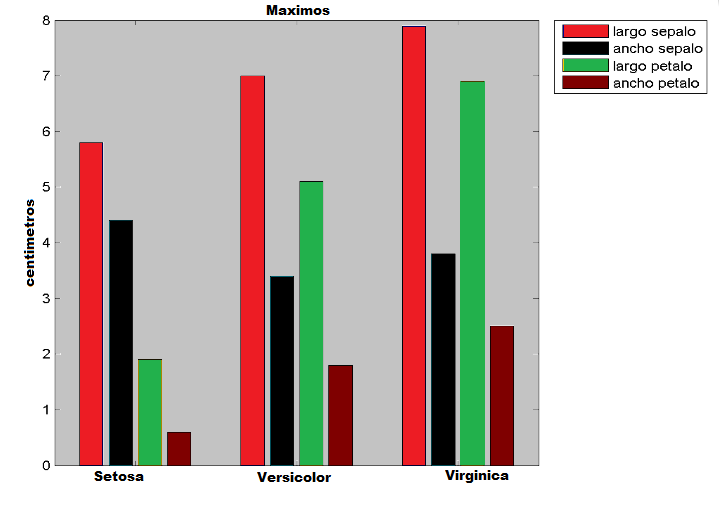
\includegraphics[scale=0.5]{maximos}\caption{Máximos valores alcanzados por cada tipo de Lirio}
\end{figure}



\begin{figure}[H]
\hspace{2cm}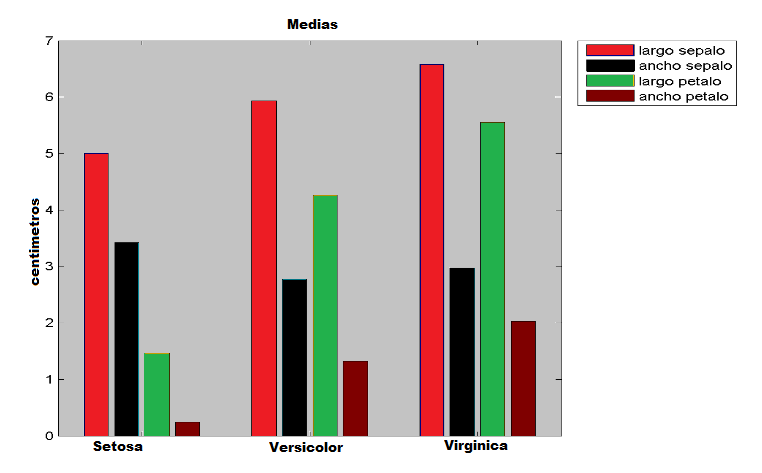
\includegraphics[scale=0.5]{medias}\caption{Medias alcanzadas por cada tipo de Lirio}
\end{figure}



\begin{figure}[H]
\hspace{2cm}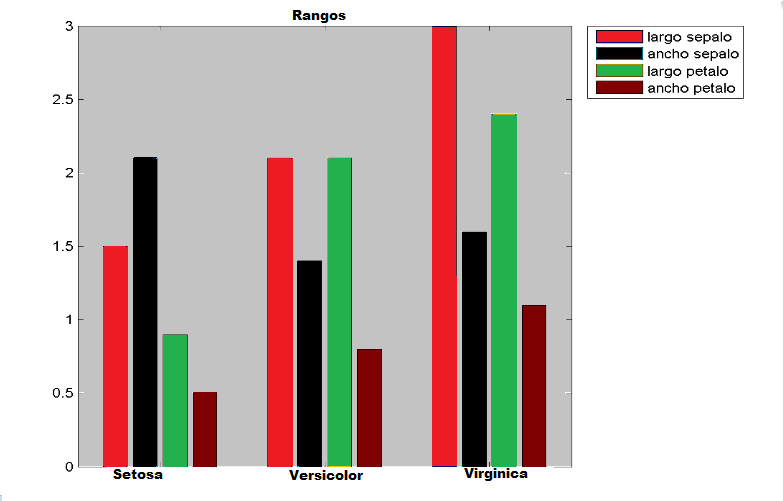
\includegraphics[scale=0.5]{rangos}\caption{Rangos alcanzados por cada tipo de Lirio}
\end{figure}


\item Gráfico de los valores:


\begin{figure}[H]
\hspace{2cm}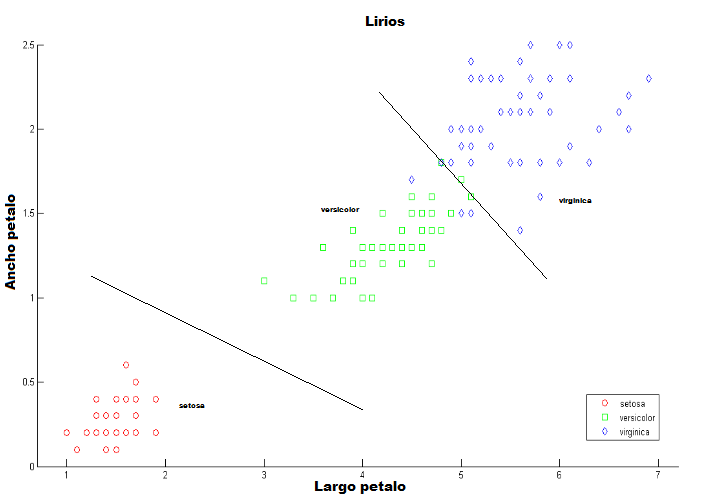
\includegraphics[scale=0.5]{anchovslargoPetalo}\caption{Posibles {}``rangos'' de valores útiles para clasificar cada lirio
a partir de las dimesiones de su pétalo}
\end{figure}



En el gráfico puede observarse que hay un umbral muy definido entre
la clase $setosa$ de Lirio frente a las otras dos. No siendo tan
así para los tipos $versicolor$ y $virg\acute{\imath}nica$. Por
lo que, a simple vista, se puede intuir que si hay errores de clasificacion,
es muy probable que sean entre estas dos especies. 

\item Asumiendo distribución gaussiana

\begin{enumerate}
\item Código\end{enumerate}
\begin{lyxcode}
load~fisheriris;

NB~=~NaiveBayes.fit(meas,species);~

NB\_Clases=NB.predict(meas);\end{lyxcode}
\begin{enumerate}
\item Porcentaje de datos mal calculados = $4\%$
\item Matríz de confusión
\end{enumerate}

\begin{tabular}{|c|c|c|}
\hline 
50 & 0 & 0\tabularnewline
\hline 
0 & 47 & 3\tabularnewline
\hline 
0 & 3 & 47\tabularnewline
\hline 
\end{tabular}


En la matríz de confusión, todos los valores que se encuentran fuera
de la diagonál principal, son valores que se clasificaron mal. A partír
de esta observación, se puede calcular el error cometido como $\frac{incorrectos}{total}=\frac{3+3}{150}=0.04$.
Un $4\%$ de error.\end{enumerate}
\end{enumerate}

\end{document}
